% Copyright (C) 2005-2015 Airbus - EDF - IMACS - Phimeca
% Permission is granted to copy, distribute and/or modify this document
% under the terms of the GNU Free Documentation License, Version 1.2
% or any later version published by the Free Software Foundation;
% with no Invariant Sections, no Front-Cover Texts, and no Back-Cover
% Texts.  A copy of the license is included in the section entitled "GNU
% Free Documentation License".
\renewcommand{\filename}{docUC_StochProc_WhiteNoise.tex}
\renewcommand{\filetitle}{UC : Creation of a White Noise}

% \HeaderNNIILevel
% \HeaderIILevel
\HeaderIIILevel


\label{whiteNoise}
\index{Stochastic Process!White Noise}


This section details first how to create and manipulate a white noise.\\

A second order white noise $\varepsilon: \Omega \times \cD \rightarrow \Rset^d$  is a stochastic process of dimension $d$ such that the covariance function $C(\vect{s},\vect{t})=\delta(\vect{t}-\vect{s})C(\vect{s},\vect{s})$ where $C(\vect{s},\vect{s})$  is the covariance matrix of the process at vertex $\vect{s}$ and $\delta$ the Kroenecker function.\\

A process $\varepsilon$ is a white noise if  all finite family of locations  $(\vect{t}_i)_{i=1, \dots, n} \in \cD$, $(\varepsilon_{\vect{t}_i})_{i=1, \dots, n}$ is independent and identically distributed.\\

OpenTURNS proposes to model it through the object  \emph{WhiteNoise} defined on a mesh  and a distribution with zero mean and finite standard deviation.\\
If the distribution has a mean different from zero, OpenTURNS sends a message to prevent the User and does not allow the creation of such a white noise.\\

\requirements{
  \begin{description}
  \item[$\bullet$] a distribution : {\itshape myDist}
  \item[type:]  Distribution
  \end{description}

  \begin{description}
  \item[$\bullet$] a mesh : {\itshape \textit{myMesh}}
  \item[type:]  Mesh
  \end{description}

}
{
  \begin{description}
  \item[$\bullet$] a white noise : {\itshape myWN}
  \item[type:]  WhiteNoise
  \end{description}
}

\textspace\\
Python script for this UseCase :

\inputscript{script_docUC_StocProc_WhiteNoise}

\textspace\\

The first example illustrated in the  Figures \ref{whitenoiseRealization} to \ref{whitenoiseRealizations} is a univariate white noise distributed according to the standard normal distribution. We draw some realizations of the time grid = $[0,99]$ with $\Delta t = 1.0$.\\


The second example illustrated in the  Figures  \ref{WNMeshRealInterpolate} and \ref{WNMeshRealNotInterpolate} is a univariate white noise distributed according to the standard normal distribution.   We draw some realizations on a mesh of dimension 2.\\
The Figures \ref{WNMeshRealInterpolate} and \ref{WNMeshRealNotInterpolate} respectively draw   one realization  of the process when the values are interpolated and not interpolated.



\begin{figure}[H]
  \begin{minipage}{9cm}
    \begin{center}
      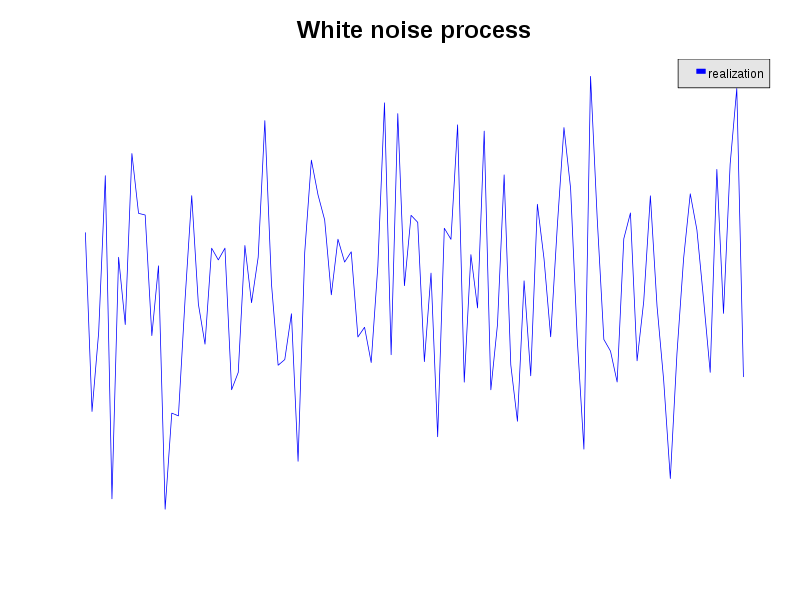
\includegraphics[width=7cm]{Figures/whitenoise_realization.png}
      \caption{Realization of a white noise with distribution $\cN(0, 1)$}
      \label{whitenoiseRealization}
    \end{center}
  \end{minipage}
  \hfill
  \begin{minipage}{9cm}
    \begin{center}
      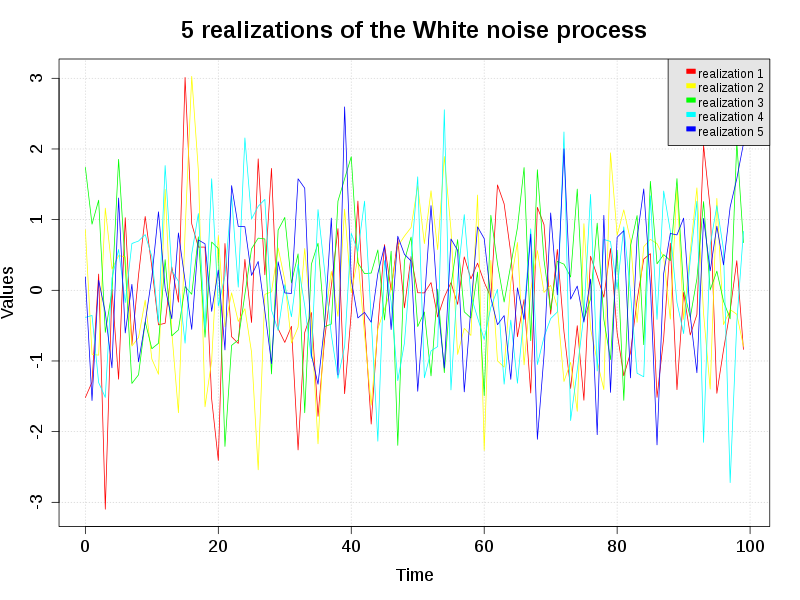
\includegraphics[width=7cm]{Figures/whitenoise_realizations.png}
      \caption{5 realizations of a white noise with distribution $\cN(0, 1)$.}
      \label{whitenoiseRealizations}
    \end{center}
  \end{minipage}
\end{figure}



\begin{figure}[H]
  \begin{minipage}{9cm}
    \begin{center}
      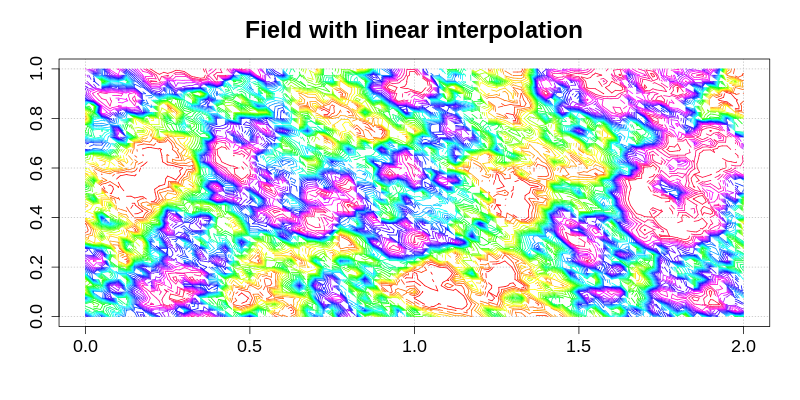
\includegraphics[width=7cm]{Figures/Field_interp.png}
      \caption{One realization of the white noise defined on the mesh with distribution $\cN(0, 1)$ when the values are interpolated.}
      \label{WNMeshRealInterpolate}
    \end{center}
  \end{minipage}
  \hfill
  \begin{minipage}{9cm}
    \begin{center}
      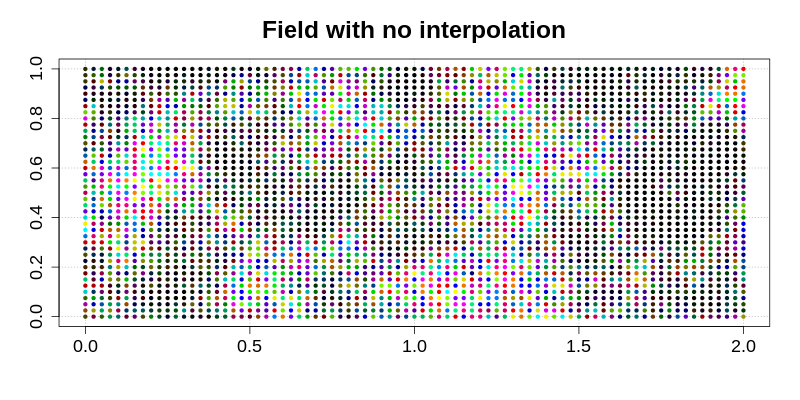
\includegraphics[width=7cm]{Figures/Field_nointerp.png}
      \caption{Previous realization of the white noise defined on the mesh with distribution $\cN(0, 1)$ when the values are not interpolated.}
      \label{WNMeshRealNotInterpolate}
    \end{center}
  \end{minipage}
\end{figure}
